
    \documentclass[journal,twoside]{IEEEtran}
    \usepackage{cite}
\usepackage[pdftex]{graphicx}
\graphicspath{{./universal/}}
\DeclareGraphicsExtensions{.png,.pdf,.jpeg,.jpg}
\usepackage{amsmath}
\usepackage{algorithmic}
\usepackage{array}
\usepackage{url}
    \begin{document}

    \setcounter{page}{48}
    \title{Universal Power Converter For
Microhydro Power Plant}
    \author{\IEEEauthorblockN{Laxman Timilsina*, Prakash Acharya, Ram Prasad Jnawali, Sushil Poudel, Indraman Tamrakar**, Netra Gyawali***}\\
    \IEEEauthorblockA{Department of Electrical Engineering, \\Institute of Engineering,\\ Tribhuvan University, Pulchowk, Lalitpur, Nepal \\
    *Email: laxmant993@gmail.com\\ **Email: im.tamrakar@hotmail.com\\ ***Email: netra@ioe.edu.np}}

\markboth{Zerone Scholar,~Vol.~1, No.~1, November~2016}%
{Timilsina \MakeLowercase{\textit{et al.}}: Universal Power Converter}
    \maketitle
	\begin{abstract}
With increasing trends of non-linear and reactive
loads even in Micro Hydro Power (MHP) Scheme, problems due
to harmonic current and reactive power balance is increasing.
The conventional Electronic Load Controller (ELC) for speed
control does not take care of effect of un-balanced consumer’s
load. The conventional ELC consumes some reactive power due
to delayed chopping of waveform of current through ballast load
of ELC. This paper proposes an advanced Electronic Universal
Controller which takes care of frequency control, reactive power
balance and voltage control, harmonic current compensation and
unbalanced load compensation by a single compensator. The
proposed system operates on the basis of instantaneous P-Q
theory by which the harmonics and neutral current is suppressed
and further the outer control scheme is applied for the frequency
balance and reactive power compensation.
	\end{abstract}
	\begin{IEEEkeywords}
Active Power Filter, Electronic Load Controller, Micro-hydro Power Plant, Non-linear Load, 
Power Quality.
	\end{IEEEkeywords}
	\section{Introduction}
Distributed power generation has received greater attention
in recent years for power supply in remote and rural
communities due to the high cost and power losses
transmission line supplying power from national grid to such
remote areas. Thus, suitable stand-alone systems using locally
available energy sources have become a preferred option.
Micro Hydro Power (MHP) scheme is one of the readily
available renewable energy sources\cite{1}.

\bigskip
The growing number of power electronics-based equipment
has produced deterioration in the power quality by introduction
of harmonics in the system network. At the same time, much of
the equipment causing the disturbances is quite sensitive to the
deviations from the ideal sinusoidal line voltage\cite{2}. The
presence of harmonics in the power lines results in greater
power losses and also in operation failures of electronic equipment, which
are more sensitive since they include microelectronic control
systems that work at lower energy levels. The high
flow of neutral current due to unbalance load in MHP scheme
is undesirable.The general trend in MHP scheme is to have ELC
for frequency control, Shunt VAR Compensator for voltage
control and Shunt Active Power Filter for harmonic
compensation as shown in Fig~\ref{f1} \cite{2}.

\begin{figure}[!ht]
\centering
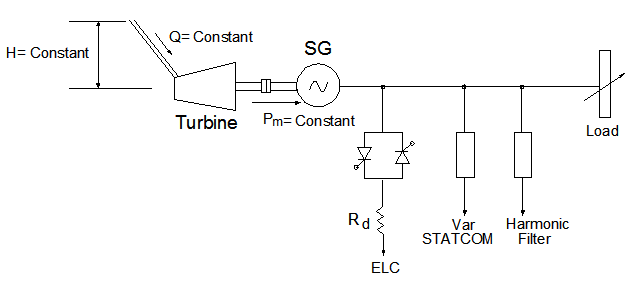
\includegraphics[width=3in]{1}
\caption{Conventional Scheme of MHP plant}
\label{f1}
\end{figure}

\bigskip
The turbine of MHP plant is generally unregulated giving
constant mechanical power input to the generator at its full
rating and active power balance is maintained by ELC by
dumping the excess of power generated to the dump load $R_d$ 
thus by controlling the frequency of generated voltage to
acceptable range. Control of voltage magnitude is another
prime concerns in MHP scheme. Shunt VAR compensators like
–Thyristor Switched Capacitors (TSC), Fixed Capacitor-
Thyristor Control Reactor (FC-TCR), STATCOM are generally
used for reactive power balance and voltage control. Active
power filter (harmonic filter) is used for harmonic current
compensation. This paper proposes an advanced Electronic
Load Controller which takes care of frequency control,
reactive power balance and voltage control, harmonic current
compensation and un-balanced load compensation by a single
compensator.
	\section{Proposed Scheme and Its Control}
Fig.~\ref{f2} shows the schematic diagram of the proposed scheme
with Universal Power Converter. The switching patterns of
power electronic switches $S_1$ to $S_7$ are controlled in such a way
that the converter branch current draws desired current to
compensate reactive power and harmonic power consumed by
the load and at the same time, dumping the proper amount of active power to the dump load $R_d $ through the chopper switch
$‘S_7 ’$ and compensating the neutral current due to unbalanced
consumer’s load. The scheme can be used for compensation of harmonic
components, unbalanced currents, reactive power and
frequency balance for the unbalanced and nonlinear load
connected across the consumer loads in a micro-hydro plant.
\begin{figure}[!ht]
\centering
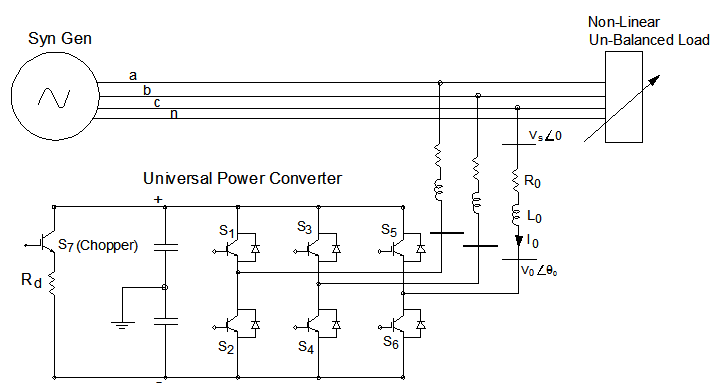
\includegraphics[width=3in]{2}
\caption{Schematic diagram of proposed scheme}
\label{f2}
\end{figure}

\bigskip
Fig.3~\ref{f3} shows the control system diagram of the proposed
scheme. The load currents and the terminal voltage of the
synchronous generator is sensed and passed to the P-Q Theory
block which generates the reference currents for harmonics,
unbalanced load compensation.
\begin{figure}[!ht]
\centering
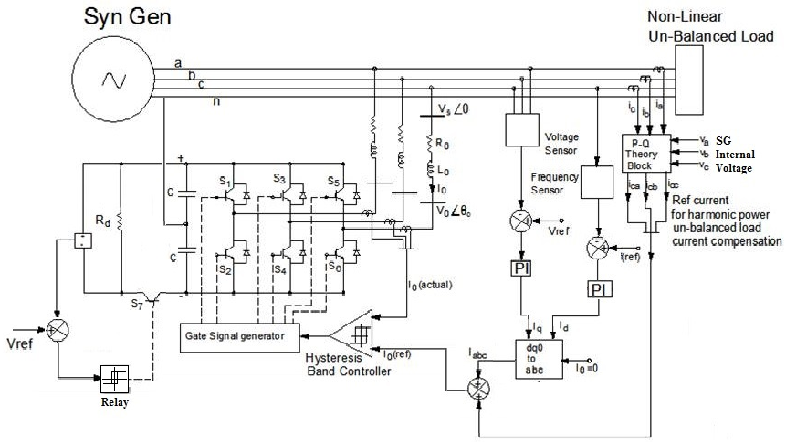
\includegraphics[width=3in]{3}
\caption{Control system diagram of proposed scheme}
\label{f3}
\end{figure}


\bigskip
The P-Q Theory formally known as “The Generalized Theory of
the Instantaneous Reactive Power in Three-Phase Circuit” was
first developed by H. Akagi in 1983. It is based on
instantaneous values in three phase power systems with or
without neutral wire, and is valid for steady state or transitory
operations, as well as for generic voltage and current
waveforms. The P-Q Theory consists of an algebraic
transformation known as a Clarke transformation of the three
phase input voltages and the load harmonic currents in the abc
coordinates to the $0-\alpha -\beta$ reference frame followed by the
calculation of the real and reactive instantaneous power
components as illustrated in Fig.~\ref{f4} and following equations:

\begin{figure}[!ht]
\centering
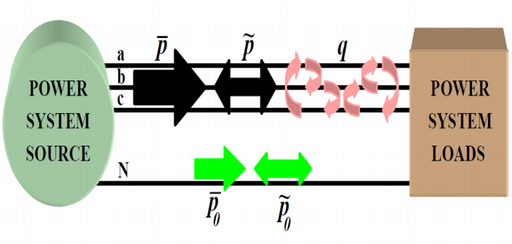
\includegraphics[width=3in]{4}
\caption{Illustration of instantaneous p-q theory}
\label{f4}
\end{figure}




\[ \begin{bmatrix} v_0 \\ v_{\alpha} \\v_{\beta} \end{bmatrix}
=\sqrt{\frac{2}{3}} \begin{bmatrix} \frac{1}{\sqrt 2} & \frac{1}{\sqrt 2} &\frac{1}{\sqrt 2}\\ 1 & \frac{-1}{2} & \frac{-1}{2}\\ 0 & \frac{\sqrt 3}{2} & \frac{-\sqrt 3}{2} \end{bmatrix} \begin{bmatrix} v_a \\ v_b \\ v_c \end{bmatrix} \] 


\[ \begin{bmatrix} i_0 \\ i_{\alpha} \\i_{\beta} \end{bmatrix}
=\sqrt{\frac{2}{3}} \begin{bmatrix} \frac{1}{\sqrt 2} & \frac{1}{\sqrt 2} &\frac{1}{\sqrt 2}\\ 1 & \frac{-1}{2} & \frac{-1}{2}\\ 0 & \frac{\sqrt 3}{2} & \frac{-\sqrt 3}{2} \end{bmatrix} \begin{bmatrix} i_a \\ i_b \\ i_c \end{bmatrix} \] 

$p_0=v_0*i_0$ Instantaneous zero-sequence power

$p= v_{\alpha}*i_{\alpha}+v_{\beta}*i_{\beta}$ Instantaneous real power

$ q= v_{\alpha}*i_{\beta}+v_{\beta}*i_{\alpha}$ Instantaneous imaginary power

%MATRIX INPUT

\[\begin{bmatrix} p\\q \end{bmatrix} =  \begin{bmatrix} v_{\alpha} & v_{\beta}\\v_{\beta} & -v_{\alpha} \end{bmatrix} \begin{bmatrix} i_{\alpha} \\i_{\beta} \end{bmatrix}
\]


$p_0$ (oscillating) is the value of the instantaneous zero
sequence power. This corresponds to the power which is
transferred from the power supply to the load through the zero
sequence components of voltage and current corresponds to the
alternating power of the instantaneous zero sequence power.
p (oscillating) is the mean value of the instantaneous real
power. This corresponds to the energy per unit time
which is transferred from the power supply to the load. This
corresponds to real power which is exchanged between the
power supply to the load. q is the instantaneous imaginary
power. This corresponds to the reactive power that is
exchanged between the phases of the load. This component is
not constructive to the system and is accountable for the
undesirable current which circulates between the system phases.


\bigskip
The frequency sensor senses the actual frequency of the
system and compares with the reference frequency of 50Hz.
The error signal thus obtained is passed through a PI controller
to obtain $i_d$ reference current. 
\begin{figure}[!ht]
\centering
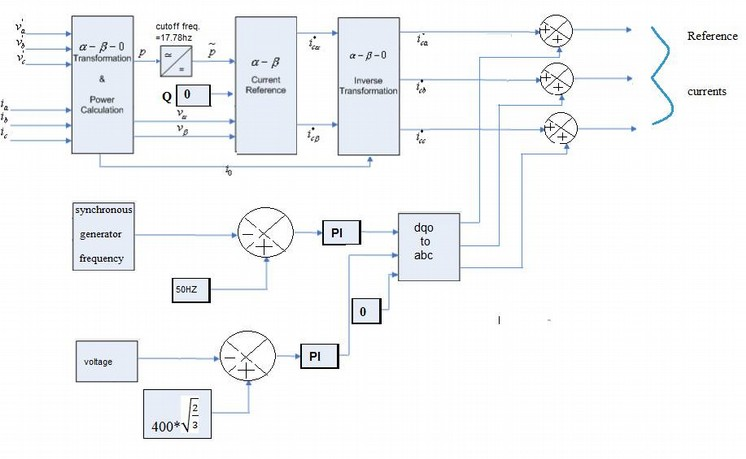
\includegraphics[width=3in]{5}
\caption{Reference current generation}
\label{f5}
\end{figure}
The voltage sensor senses the
load terminal voltage and it is compared with reference
voltage. The error signal so obtained is passed through a PI
controller to get $i_q$ reference current. Then dqo to abc
transformation is done using dq theory to obtain i abc reference
current for maintaining active and reactive power balance. The
reference current generated by p-q theory block is added up to
get final reference current ‘ $i_{abc}$ ’ as shown in Fig~\ref{f5} . Now, the
final reference current $i_{abc}$ is compared with actual current in
the hysteresis band controller. The hysteresis band controller
generates the gate signals for inverter switches so that the
actual inverter branch current tracks the reference current
within specified bands. The dc side of the inverter has two
identical dc link capacitors whose midpoint is connected to the
neutral of the ac mains. The average voltage across the dc link
capacitors is always maintained to about 600V by controlling
the duty cycle of chopper switch $S_7$ so that excess of active
power generated is dump to the ballast load $R_d$.
	


\section{Modelling of Proposed Scheme}


\begin{figure}[!ht]
\centering
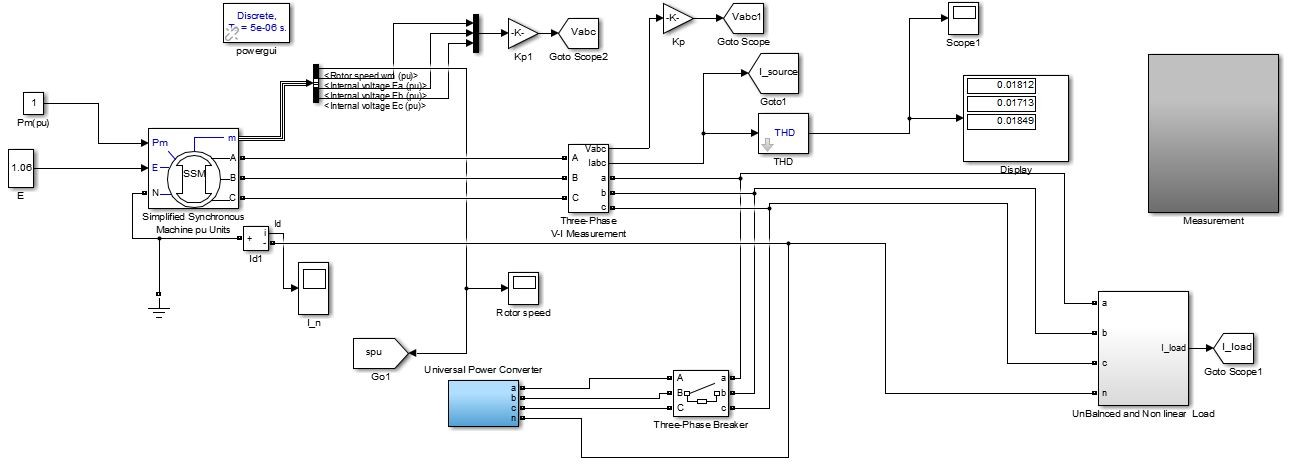
\includegraphics[height=3in,width=6in, angle =90]{6}
\caption{Overall Simulink model of Proposed Scheme}
\label{f6}
\end{figure}

Fig.~\ref{f6} shows the overall simulink simulation model of the
proposed scheme. A 16kVA synchronous generator model with
constant mechanical power input of 1 p.u. is used to represent
MHP generator. The dc excitation input voltage is set 1.06 p.u,
which is just sufficient to generate rated voltage at no-load and
purely resistive load. The non-linear un-balanced load is
simulated by R-L load supplied through the diode rectifier as
shown in Fig.~\ref{f7}

\begin{figure}[!ht]
\centering
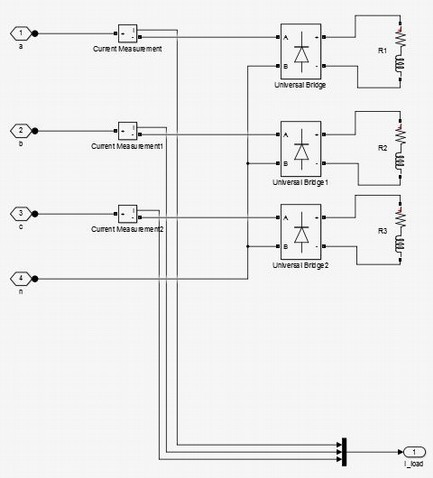
\includegraphics[width=3in]{7}
\caption{Representation of 3- $\phi$ unbalanced non linear load}
\label{f7}
\end{figure}
Fig.~\ref{f8}shows the detail of universal power converter block. The
reference current generated by instantaneous p-q block is
compared with the actual inverter branch current in the
hysteresis band controller as shown in Fig.~\ref{f9}

\begin{figure}[!ht]
\centering
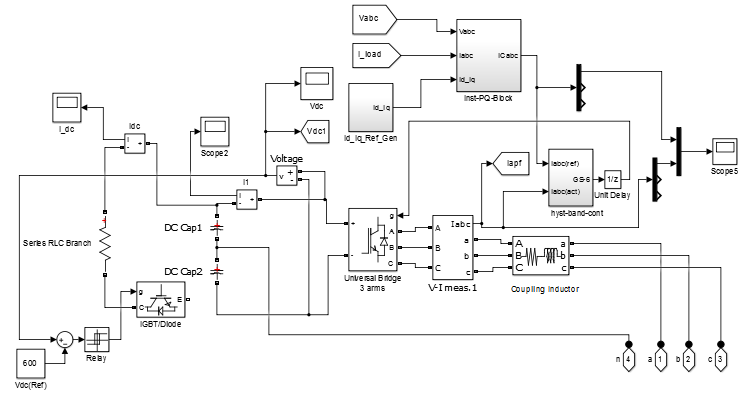
\includegraphics[width=3in]{8}
\caption{Detail of universal power converter block}
\label{f8}
\end{figure}

\begin{figure}[!ht]
\centering

\includegraphics[width=3in]{9}
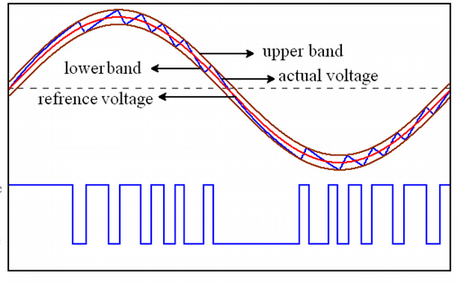
\includegraphics[width=3in]{99}
\caption{Hysteresis band current controller}
\label{f9}
\end{figure}

\bigskip
It is an instantaneous feedback current control method in
which a band is created around a reference current. The
reference current is the required current that is expected to be
injected by the inverter ideally. The hysteresis band provides
boundary around reference current within which the actual
inverter branch current is made to track. The instantaneous
injected current from the inverter ( $i_0$ ) and reference current
generated ( $i_{ref}$ ) is supplied as input to the block and accordingly
hysteresis band of the current is created. The relay is
configured with the switch on point as 0.1 and switch off point
as -0.1. Hence, the relay creates a hysteresis band and checks if
the injected current is within the band. Thus, the relay
generates gate signals in following pattern:
When $i_{abc(act)}$ – $i_0$ ≤ -0.1, output of relay =1
When $i_{abc(ref)}$ – $i_0$ ≥ 0.1, output of relay =0
With this logic, the hysteresis band current controller generates
the gate signals of IGBT switch pair of the inverter so that the actual inverter branch current tracks the reference current
within specified bands.

\section{Simulation Results}
The complete simulation model shown in the Fig.~\ref{f6} is run for
time span of 2 seconds. The universal power converter branch
is switched on after 0.5 sec to observe responses of the scheme
before and after the connection of the universal power
converter. The followings are the rating and parameters of the
components used in the simulation.


\bigskip
Synchronous generator:\\
16 kVA, 400V, 50 HZ, 1500 rpm\\
Un-balanced non-liner Load:\\
R-L series load supplied through diode rectifier with\\
R=10$\Omega$, L = 0.1H for phase-A\\
R=15$\Omega$, L = 0.1H for phase-B\\
R=5$\Omega$, L = 0.1H for phase-C\\
Coupling inductor:\\
L = 2 mH, R = 0.2 Ω\\
DC link capacitors: 1000 μF each\\



\bigskip
Then the simulation results are as follows:

\begin{figure}[!ht]
\centering
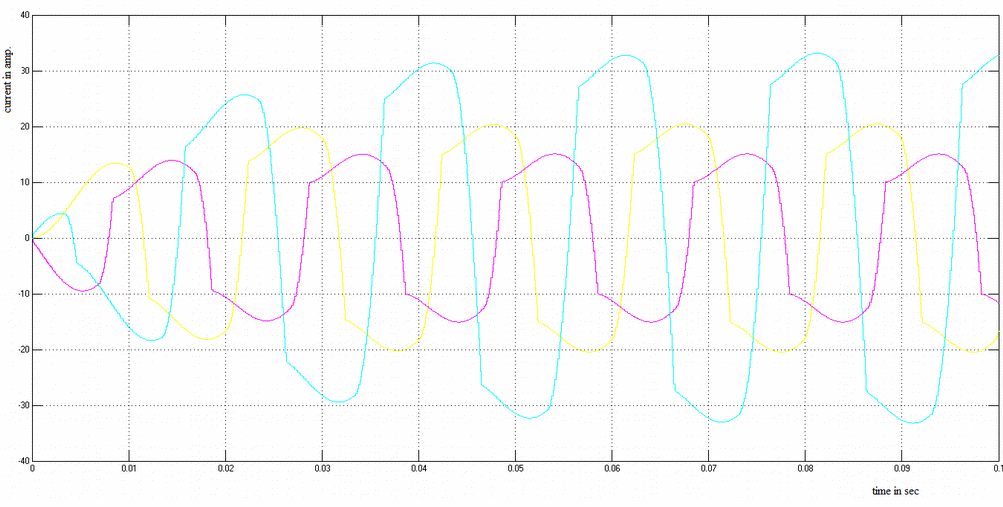
\includegraphics[width=3in]{10}
\caption{Waveform of current drawn by load}
\label{f10}
\end{figure}

\begin{figure}[!ht]
\centering
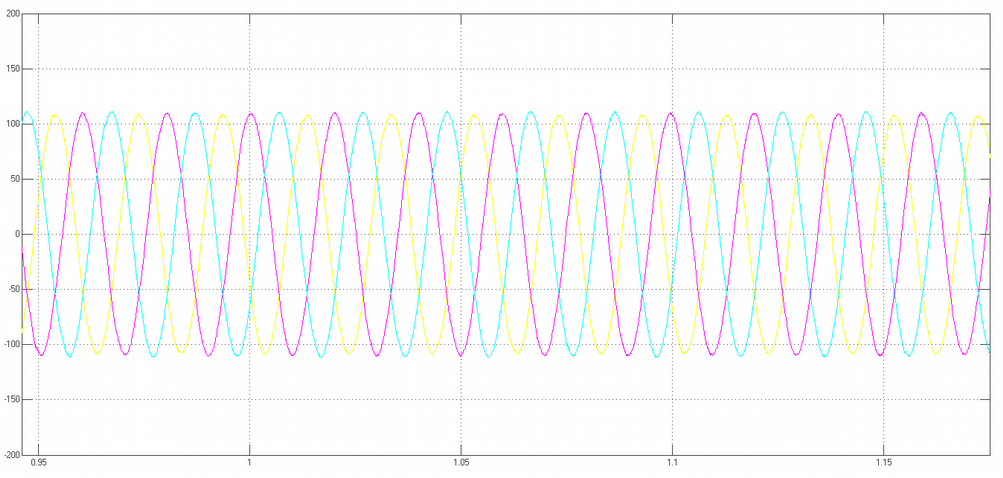
\includegraphics[width=3in]{11}
\caption{Waveform of source current after compensation}
\label{f11}
\end{figure}

\begin{figure}[!ht]
\centering
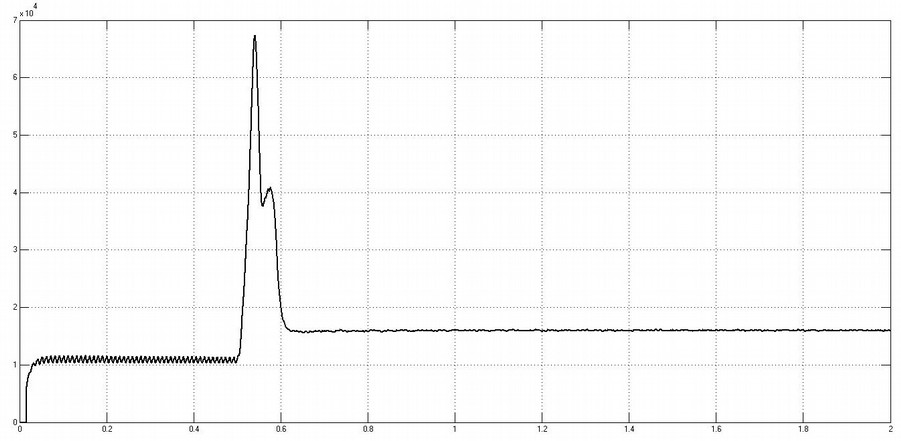
\includegraphics[width=3in]{12}
\caption{Active power consumed by load}
\label{f12}
\end{figure}

\begin{figure}[!ht]
\centering
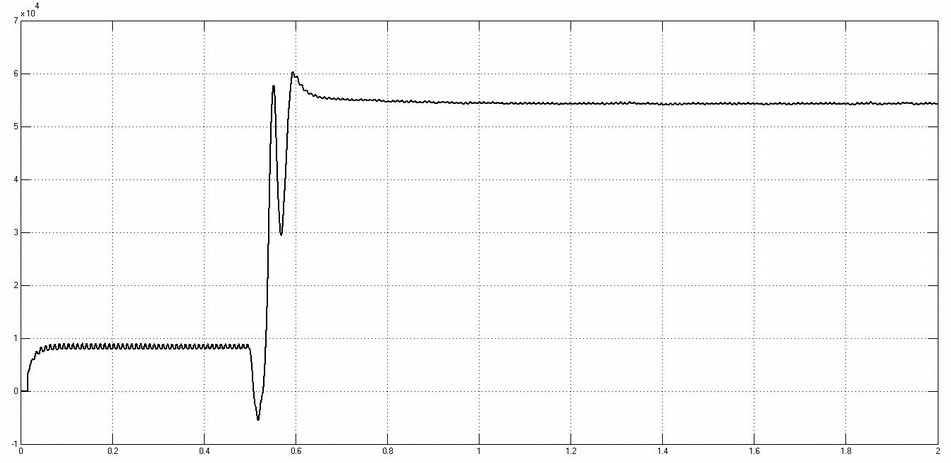
\includegraphics[width=3in]{13}
\caption{Reactive power consumed by load}
\label{f13}
\end{figure}

\begin{figure}[!ht]
\centering
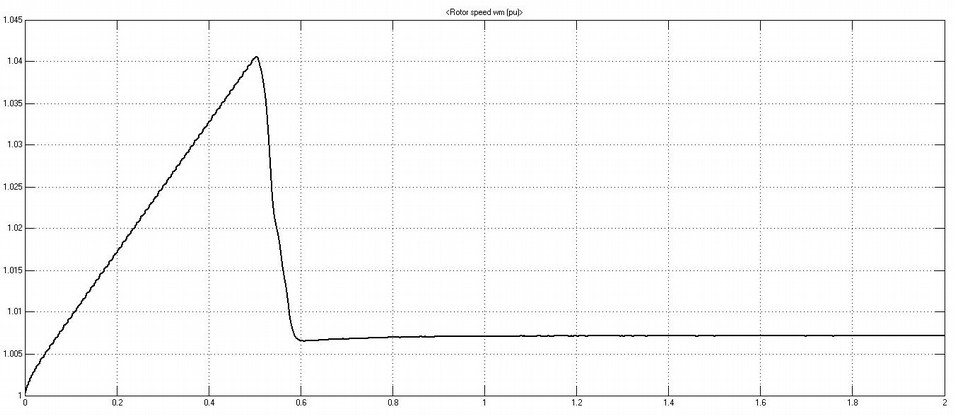
\includegraphics[width=3in]{14}
\caption{Waveform of neutral currnet before and after compensation}
\label{f14}
\end{figure}

\begin{figure}[!ht]
\centering
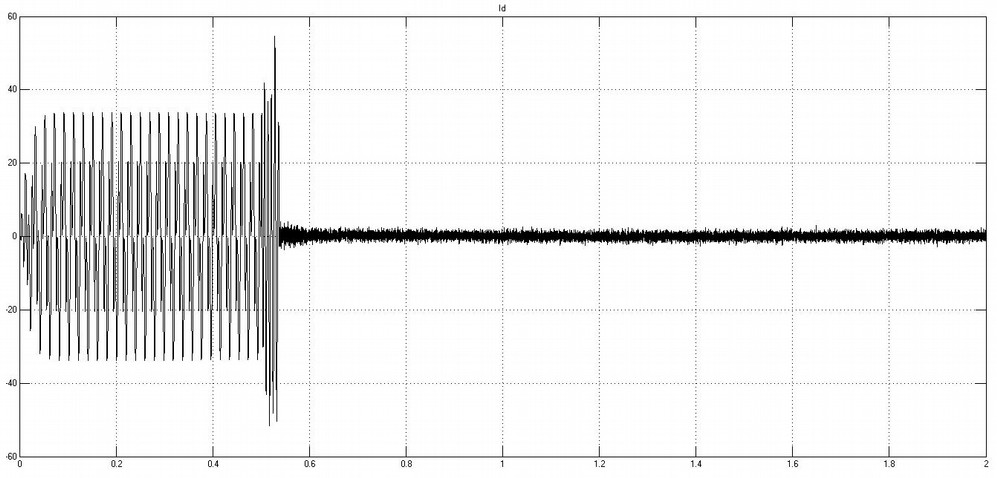
\includegraphics[width=3in]{15}
\caption{Rotor Speed Response}
\label{f15}
\end{figure}


\bigskip

Fig.~\ref{f10} shows the waveforms of load currents, which in unbalanced and non-sinusoidal due to the un-balanced non-
linear load. In the absence of universal power compensator,
the synchronous generator is bound to supply these unbalanced non-sinusoidal currents. Fig.~\ref{f11} shows the
waveforms of current supplied by the synchronous generator
after connecting the universal power converter. The three
phase currents are balanced and nearly sinusoidal. It is clear from the Fig.~\ref{f12} that the magnitude of neutral current
of the generator is very significant before compensation and
it very small after compensation. Fig.~\ref{f13} and Fig.~\ref{f14} shows
the active power consumed by the load and reactive power
consumed by the load respectively. Fig.~\ref{f15} shows the speed
response of the synchronous generator, which shows that the
speed is uncontrolled before connecting the Universal Power
Converter and it is well controlled to nearly 1pu after
connecting the Universal Power Converter.
\section{Conclusion}

The proposed scheme of Universal Power Converter is
successfully simulated in the MATLAB Simulink. The
proposed controller takes care of frequency control, reactive
power balance and voltage control, harmonic current
compensation and un-balanced load compensation by a
single compensator. The proposed system operates on the
basis of instantaneous p-q theory by which the harmonics
and neutral current is suppressed and further the outer
control scheme is applied for the frequency balance and
reactive power compensation. With the implementation of
this scheme the harmonic and unbalanced current of the
generator has significantly reduced. The simulation results
shows that the Total Harmonic Distortion (THD) of the
source current has reduced from 35\% to 2.5\%. The active
power balance and reactive power balance has been
maintained thus by resulting constant speed operation and
constant terminal voltage magnitude to respective rated
values.

\begin{thebibliography}{9}

\bibitem{1} H. Akagi, Y. Kanazawa, A. Nabae, \emph{Generalized Theory of the
Instantaneous Reactive Power in Three-Phase Circuits},
IPEC'83 - Int. Power Electronics Conf., Tokyo, Japan, 1983,
pp. 1375-1386.

\bibitem{2} Rashid, M. H. (Ed). \emph{Power Electronics Handbook: Devices,
Circuits, and Applications}, 3rd Ed, Butterworth-Heinemann
Publishers, 2011, pp.1193-1228

\bibitem{3} H. Akagi, E.Watanabe, M. Aredes, IEEE press, \emph{Instantaneous
Power Theory and Applications to power conditioning}.

\bibitem{4} Juan
W. Dixon, J.J. Garcia, and Luis Moran, \emph{Control
System For Three-Phase Active Power Filter Which
Simultaneously Compensates Power Factor
and
Unbalanced
Loads}, IEEE Trans. Ind. Electron.Vol.42,
No.6, 1995.

\bibitem{5} Li Bin, Tong Minyong, \emph{Control Method of the Three-Phase
Four-Leg Shunt Active Power Filter}, Energy Procedia , vol.
14, 2012, pp.1825–1830.

\end{thebibliography}
\begin{IEEEbiography}[{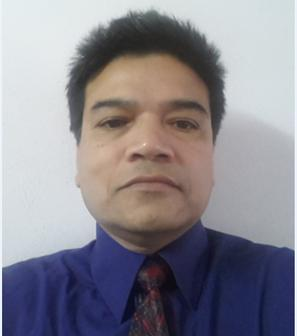
\includegraphics[width=1in,height=1.25in,clip,keepaspectratio]{imt}}]{Indraman Tamrakar}
was born in
Kathmandu, Nepal, in 1958. He received the Bachelor's degree in
Electrical Engineering from the Punjab University, Chandigarh, India, in 1983, M.sc. Engg from University of
Calgary, Canada in 1992 and Ph.D. degrees in electrical
engineering from Tribhuvan University, Nepal in 2007. In
1983, he joined the Department of Electrical
Engineering, Pulchowk campus, IOE as a
Lecturer, and in 1997 became a Reader and
Professor in 2005. His current research interests
include Power Electronics, electrical Machines
Flexible AC Transmission Systems and Renewable
Energy Technology. Dr. Tamrakar has served as
Head of Department in Department of Electrical
Engineering, Pulchowk campus, IoE for several
terms.
\end{IEEEbiography}
\vspace{-2cm}
\begin{IEEEbiography}[{
\includegraphics[width=1in,height=1.25in,clip,keepaspectratio]{ng}}]{Netra Prasad Gyawali}
 received the
Bachelor's degree in electrical engineering
from the Tribhuvan University,
Institute of Engineering, Pulchowk
Campus. He is currently working as M.Sc. Program Co-ordinator at Department of Electrical Engineering, Pulchowk Campus, IoE, Pulchowk, Lalitpur.

\end{IEEEbiography}
\vspace{-2cm}

\begin{IEEEbiography}[{
\includegraphics[width=1in,height=1.25in,clip,keepaspectratio]{lt}}]{Laxman Timilsina}
was born in Kaskikot 9,
Kaski in November 1993 AD. He is currently studying B.E. in Electrical Engineering in
Tribhuwan University, IoE, Pulchowk Campus. His fields of
interest are Control system, Electric Machines, Power System
and Demand Side Management.
\end{IEEEbiography}
\vspace{-2cm}
\begin{IEEEbiography}[{
\includegraphics[width=1in,height=1.25in,clip,keepaspectratio]{rpj}}]{Ram P. Jnawali}
was born in May 13,
1995. He is currently studying Bachelor in Electrical Engineering
at Pulchowk Campus, IOE, Pulchowk. His fields of interests are
Power Systems, Electrical machines, Energy economics and
Energy system management.
\end{IEEEbiography}
\vspace{-2cm}
\begin{IEEEbiography}[{
\includegraphics[width=1in,height=1.25in,clip,keepaspectratio]{sp}}]{Sushil Paudel}
was born in September 18,
1995. He is currently studying Bachelor in Electrical Engineering
at Pulchowk Campus, IOE, Pulchowk. His fields of interests are
Power Systems, FACTS, Control Systems, and solid-state power
converter design and control.
\end{IEEEbiography}
\vspace{-2cm}
\begin{IEEEbiography}[{
\includegraphics[width=1in,height=1.25in,clip,keepaspectratio]{pa}}]{Prakash Acharya}
was born in September, 5
1994. He is currently studying Bachelor in
Electrical Engineering at Pulchowk Campus,
IOE, Pulchowk. His fields of interests are
Power Systems, FACTS, Power quality,
Control Systems, and solid-state power
converter design and control.
\end{IEEEbiography}



\end{document}

